\documentclass[fontsize=10.5pt]{jlreq}

%---If you use beamer class, add aspectratio=169 and change jlreq to beamer---%

%---Package part---%
\usepackage{amssymb,amsmath,amsthm,amscd}
\usepackage{ascmac}
\usepackage{bm}
\usepackage{color}
\usepackage{circuitikz}
\usepackage{derivative}
\usepackage{enumitem} % If you use beamer metropolis, ignore this package
\usepackage{fancybox}
\usepackage{frame,framed}
\usepackage{float}
\usepackage{graphicx}
\usepackage{mathtools}
\usepackage{physics2}
\usepackage{pgfplots}
\usepackage{siunitx}
\usepackage{tabularray}
\usepackage{tcolorbox}
\usepackage{tikz}
\usepackage{url}
\usepackage{titlepic} % If you use beamer metropolis, ignore this package
\usepackage{wrapfig}
%---Package part END---%

%---Package Module part---%
\usephysicsmodule{ab,braket,doubleprod,xmat}
\pgfplotsset{compat=1.18}
%---Package Module part END---%

%---Cont foot nad head settings---%
\DefTblrTemplate{contfoot-text}{normal}{（次ページに続く）}
\SetTblrTemplate{contfoot-text}{normal}
\DefTblrTemplate{conthead-text}{normal}{（続き）}
\SetTblrTemplate{conthead-text}{normal}
%---Cont foot nad head settings END---%

%---For equation number part---%
\usepackage[hang,small,bf]{caption}
\usepackage[subrefformat=parens]{subcaption}
\captionsetup{compatibility=false}
\renewcommand{\theequation}{\thesection.\arabic{equation}}
\makeatletter
\@addtoreset{equation}{section}
\makeatother
%---For equation number part END---%

%---For beamer settings part---%
%---If you use beamer metropolis,remove header % from below sentense---%
% \usepackage[haranoaji,deluxe]{luatexja-preset}% Font setting
% \usepackage{luatexja}% For use japanese
% \renewcommand{\kanjifamilydefault}{\gtdefault}% Setting normal font to gothic
% \usetheme[block=fill]{metropolis}% For use metropolis theme
%---For beamer settings part END---%

\begin{document}

\title{交流回路 Introduction}
\author{平山大知}
\date{\today}
\maketitle
\tableofcontents
\clearpage
\section{交流回路とは}
まず我々は直流回路を知っている。直流回路は電流の向きと電圧が一定な回路である。対して交流回路は電流の向きや電圧が一定周期で変化する回路である。直流回路は``Direct Current''の頭文字からDC回路、交流回路は``Alternating Current''の頭文字からAC回路と呼ばれる。

交流回路の最も身近な例は家庭用コンセントである。コンセント電圧の時間変化を測定すると周波数が\qty{50}{Hz}\footnote{もし読者が関西圏にいるならば、それは\qty{60}{Hz}である。}の正弦波に近い波形が得られる。
\begin{figure}
    \centering
    \begin{minipage}{0.48\linewidth}
        \centering
        \begin{tikzpicture}[transform shape]
	        % Paths, nodes and wires:
	        \draw (4, 10) to[battery1] (4, 6);
	        \draw (4, 10) to[short] (8, 10);
	        \draw (4, 6) to[short] (8, 6);
	        \draw (8, 10) to[american resistor] (8, 6);
        \end{tikzpicture}
        \caption{直流回路の例}
        \label{fig.直流回路の例}
    \end{minipage}
    \begin{minipage}{0.48\linewidth}
        \centering
        \begin{tikzpicture}[transform shape]
	        % Paths, nodes and wires:
	        \draw (4, 10) to[short] (8, 10);
	        \draw (4, 6) to[short] (8, 6);
	        \draw (8, 10) to[american resistor] (8, 6);
	        \draw (4, 10) to[sinusoidal voltage source] (4, 6);
        \end{tikzpicture}
        \caption{交流回路の例}
        \label{fig.交流回路の例}
    \end{minipage}
\end{figure}

なお交流回路の電源(電圧源)は図\ref{fig.交流回路の例}のように丸の中に波線を引いた記号で表される。
\section{正弦波交流回路}
交流回路のなかでも特に簡単な正弦波交流回路についてまず説明していく。
\subsection{正弦波交流回路の簡単なイメージ}
電気に全く関係なく、一般的な波の表式は以下のとおりである。
\begin{equation}
    y=A\sin\ab(a x + b)
\end{equation}
これが電気、交流回路の信号に対応するとき次のようになる。
\[V = V_{0}\sin\ab(\omega t + \alpha)\]
ここに\(V\)が電圧であり、\(V_0\)は定数、\(\omega\)が角振動数、\(\alpha\)が初期位相である。
\begin{figure}[htbp]
    \centering
    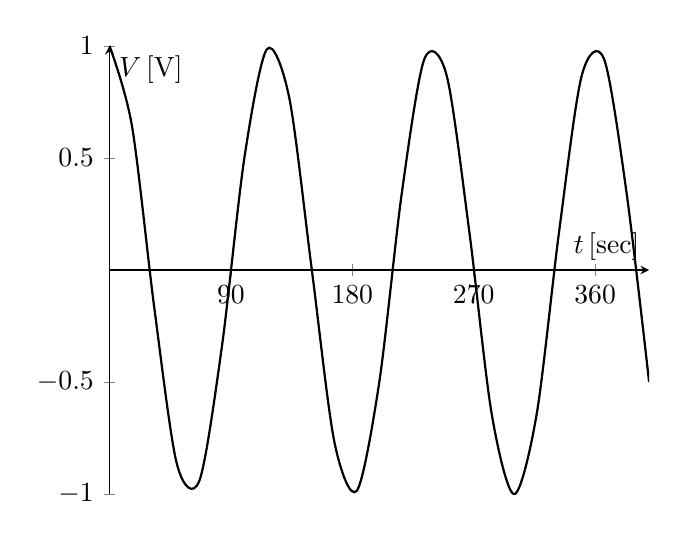
\begin{tikzpicture}
        \begin{axis}[
            axis lines = center, xtick = {-360, -270,...,360},
            xlabel = {\(t\)\,[\unit{sec}]},
            ylabel = {\(V\)\,[\unit{\volt}]}
            ]
            \addplot [domain = 0:400, thick, smooth]
            { cos(3.0*x) };
        \end{axis}
    \end{tikzpicture}
    \caption{正弦波交流回路のグラフの例}
    \label{fig.ac_circuit_graph}
\end{figure}
これは直接電圧源にオシロスコープをつなぐことを考えた波形であるが、実際の回路には抵抗器、キャパシタ(コンデンサ)、インダクタ(コイル)の要素が必ず存在する。これらの直流回路における振る舞いは既知のものであるが、交流回路における振る舞いをここから説明していこう。
\subsection{波の複素表記}
ここでまず交流回路を説明するときに非常に強力な複素表記を導入する。

まず
\begin{equation}
    \exp(j\theta) = \cos\theta + j\sin\theta
\end{equation}
は既知であるとする\footnote{回路分野では虚数単位\(i\)をしばしば\(j\)で表記する。}。これの実部と虚部を各々みると、虚部が\(\sin \theta\)でこれを上手につかえばよく交流信号が議論できそうである。

左辺のネイピア数のべきが強力であることはいうまでもないだろう。さて、では先程の形をこれで表すことを考えていく。
\begin{align}
    \exp(j\omega t) &= \cos \omega t + j \sin \omega t \\
    V_0\exp(j(\omega t + \alpha)) &= V_0(\cos (\omega t + \alpha) + j \sin (\omega t + \alpha)) \\
    V_0\exp(j\omega t)\exp(j\alpha) &= V_0(\cos (\omega t + \alpha) + j \sin (\omega t + \alpha))
    \intertext{これの虚部をとる操作をすれば結局元々の形が得られる、虚部をとる操作は\(\Im\)という記号で表す。書くときには単に\(\mathrm{Im}\)と書いても良い。}
    \Im (V_0\exp(j\omega t)\exp(j\alpha)) &= \Im (V_0(\cos (\omega t + \alpha) + j \sin (\omega t + \alpha)))\\
    \Im (V_0\exp(j\omega t)\exp(j\alpha)) &= V_0 \sin (\omega t + \alpha)
    \intertext{ここで\(V_0\exp(j\alpha)\)を\(\dot{V}\)と表す(複素数であると示すときにこのように書くこともある。時間微分ではない)と}
    \Im(\dot{V}\exp(j\omega t)) &= V_0\sin(\omega t + \alpha)\label{eq.フェーザ表示の式} \\
    &= v(t)
\end{align}
この\(\dot{V}=V_0\exp(j\alpha)\)を\textbf{フェーザ}という、また\(v(t)\)は時刻\(t\)での電圧の値である。この\ref{eq.フェーザ表示の式}式の左辺が複素平面でどのような動きをするのかを考える。

まず\(\dot{V}\)について、これは半径\(V_0\)の円周上にあって、偏角が\(\alpha\)の複素数なのでベクトルで書くことができる。そして\(\exp(j\omega t)\)については、これを掛けることは、ベクトルを原点中心に回転させることに対応している、そしてその角振動数は\(\omega\)である。つまり複素平面上において、\ref{eq.フェーザ表示の式}式の左辺は、ベクトル\(\dot{V}\)が角振動数\(\omega\)で回転している状態である。虚軸側にこれを射影してやれば正弦波曲線が偉られるわけである。

このフェーザを用いると色々と議論が簡単になる。

まずフェーザについて、オーム則が直流回路と同様にして成立している。
\begin{equation}
    \dot{V} = R\dot{I} \label{eq.オーム則}
\end{equation}
抵抗値\(R\)は実数であるので電流についても複素数、つまり先程の電圧のフェーザのように電流のフェーザも存在する。
\begin{align}
    \dot{I} &= \dfrac{V_0}{R}\exp(j\alpha) \\
    i(t) &= \Im(\dot{I}\exp(j\omega t))
\end{align}

またフェーザについてはキルヒホッフ則が直流回路と同様にして成立する。
\begin{figure}
    \centering
    \begin{minipage}{0.48\linewidth}
        \centering
    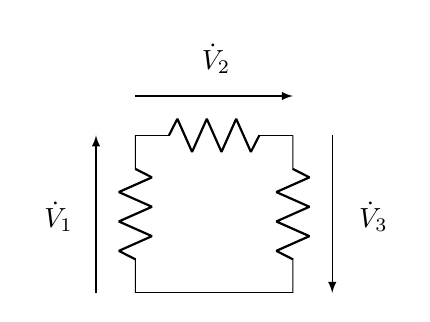
\begin{tikzpicture}[transform shape]
	    % Paths, nodes and wires:
	    \draw (3, 10) to[american resistor] (3, 8);
	    \draw (5, 10) to[american resistor] (5, 8);
	    \draw (5, 10) to[american resistor] (3, 10);
	    \draw (3, 8) to[short] (5, 8);
	    \draw[-latex] (2.5, 8) -- (2.5, 10);
	    \draw[-latex] (3, 10.5) -- (5, 10.5);
	    \draw[-latex] (5.5, 10) -- (5.5, 8);
	    \node[shape=rectangle, minimum width=0.715cm, minimum height=0.715cm] at (2, 9){} node[anchor=north west, align=left, text width=0.327cm, inner sep=6pt] at (1.625, 9.375){$\dot{V}_{1}$};
	    \node[shape=rectangle, minimum width=0.715cm, minimum height=0.715cm] at (6, 9){} node[anchor=north west, align=left, text width=0.327cm, inner sep=6pt] at (5.625, 9.375){$\dot{V}_{3}$};
	    \node[shape=rectangle, minimum width=0.715cm, minimum height=0.715cm] at (4, 11){} node[anchor=north west, align=left, text width=0.327cm, inner sep=6pt] at (3.625, 11.375){$\dot{V}_{2}$};
    \end{tikzpicture}
    \[\sum_{i}\dot{V}_{i} = 0\]
    \caption{キルヒホッフの電圧則}
    \label{fig.キルヒホッフの電圧則}
    \end{minipage}
    \begin{minipage}{0.48\linewidth}
        \centering
        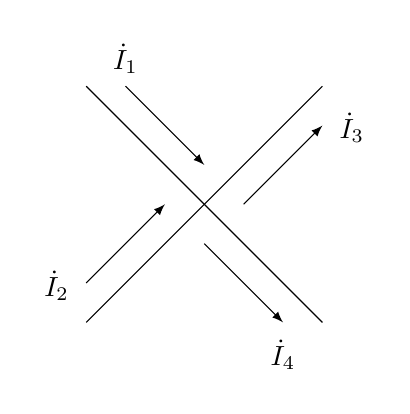
\begin{tikzpicture}[transform shape]
	% Paths, nodes and wires:
	\draw (1, 4) to[short] (2.5, 2.5);
	\draw (2.5, 2.5) to[short] (4, 4);
	\draw (2.5, 2.5) to[short] (1, 1);
	\draw (2.5, 2.5) to[short] (4, 1);
	\draw[-latex] (1.5, 4) -- (2.5, 3);
	\draw[-latex] (2.5, 2) -- (3.5, 1);
	\draw[-latex] (1, 1.5) -- (2, 2.5);
	\draw[-latex] (3, 2.5) -- (4, 3.5);
	\node[shape=rectangle, minimum width=0.715cm, minimum height=0.715cm] at (1.5, 4.375){} node[anchor=north west, align=left, text width=0.327cm, inner sep=6pt] at (1.125, 4.75){$\dot{I}_1$};
	\node[shape=rectangle, minimum width=0.715cm, minimum height=0.715cm] at (4.375, 3.5){} node[anchor=north west, align=left, text width=0.327cm, inner sep=6pt] at (4, 3.875){$\dot{I}_3$};
	\node[shape=rectangle, minimum width=0.715cm, minimum height=0.715cm] at (0.625, 1.5){} node[anchor=north west, align=left, text width=0.327cm, inner sep=6pt] at (0.25, 1.875){$\dot{I}_2$};
	\node[shape=rectangle, minimum width=0.715cm, minimum height=0.715cm] at (3.5, 0.625){} node[anchor=north west, align=left, text width=0.327cm, inner sep=6pt] at (3.125, 1){$\dot{I}_4$};
\end{tikzpicture}
    \[\sum_{i}\dot{I}_{i} = 0\]
    \caption{キルヒホッフの電流則}
    \label{fig.キルヒホッフの電流則}
    \end{minipage}
\end{figure}
\subsection{線型素子}
次に回路部品の話をする。基本的回路部品は抵抗器とキャパシタとインダクタである。抵抗器のオーム則については\ref{eq.オーム則}式で触れたので、インダクタとキャパシタについてを触れていく。
\subsubsection{インダクタ}
インダクタでは
\begin{equation}
    v(t) = L \odv{i}{t} \label{eq.インダクタの基本式}
\end{equation}
が成立している。これを操作していく。\ref{eq.インダクタの基本式}を書き下していくと
\begin{align}
    \Im(\dot{V}\exp(j\omega t)) &= L \odv{}{t}\Im(\dot{I}\exp(j\omega t))
    \intertext{一度、虚部としてではなく複素数としてみてみる}
    \dot{V}\exp(j\omega t) &= L \odv{}{t}\dot{I}\exp(j\omega t) \\
    \dot{V}\exp(j\omega t) &= j\omega L\dot{I}\exp(j\omega t) \\
    \dot{V} &= j\omega L\dot{I} \label{eq.インダクタのインピーダンス}
\end{align}
これはオーム則\ref{eq.オーム則}式と同様の形になっている。ここで抵抗のように見えるものは\(j \omega L\)である。このように拡張された抵抗概念を\textbf{インピーダンス}という。インピーダンスはしばしば\(Z\)で表される。

また位相について見てみると\ref{eq.インダクタのインピーダンス}式より\(\dot{V}\)に対して\(\dot{I}\)には\(j\)が作用しているのが見て取れる。\(j = \exp(i \tfrac{\pi}{2})\)であるから、\(\dot{V}\)に対して\(\dot{I}\)は位相が\(\tfrac{\pi}{2}\)だけ遅れている。
\subsubsection{キャパシタ}
インダクタでは
\begin{equation}
    v(t) = \dfrac{1}{C} \int i(t) \odif{t} \label{eq.キャパシタの基本式}
\end{equation}
が成立している。これを操作していく。\ref{eq.キャパシタの基本式}を書き下していくと
\begin{align}
    \Im(\dot{V}\exp(j\omega t)) &= \dfrac{1}{C}\int \Im(\dot{I}\exp(j\omega t)) \odif{t}
    \intertext{一度、虚部としてではなく複素数としてみてみる}
    \dot{V}\exp(j\omega t) &= \dfrac{1}{C}\int \dot{I}\exp(j\omega t) \odif{t} \\
    \dot{V}\exp(j\omega t) &= \dfrac{1}{j\omega C}\dot{I}\exp(j\omega t) \\
    \dot{V} &= \dfrac{1}{j\omega C}\dot{I} \label{eq.キャパシタのインピーダンス}
\end{align}
インダクタと同様に\ref{eq.キャパシタのインピーダンス}式を見てみると、キャパシタのインピーダンス\(Z_C\)は\(\tfrac{1}{j \omega C}=\tfrac{1}{\omega C}\exp\ab(-j\tfrac{\pi}{2})\)である。

位相を見てみると、\ref{eq.キャパシタのインピーダンス}式より\(\dot{V}\)に対して\(\dot{I}\)には\(\tfrac{1}{j}=-j=\exp\ab(j(-\tfrac{\pi}{2}))\)が作用しているのが見て取れる。つまり、\(\dot{V}\)に対して\(\dot{I}\)は位相が\(\tfrac{\pi}{2}\)だけ進んでいる。
\subsection{フィルター回路}
抵抗器、インダクタ、キャパシタのそれぞれを特性を用いることで、交流回路について周波数に応じて動作を変えることができる。ここではローパスフィルター(LPF)、ハイパスフィルター(HPF)、共振回路を取り上げて説明していく。
\subsubsection{ローパスフィルター(LPF)}
ローパスフィルターには様々な種類があるが、抵抗器とキャパシタを用いるものについてまず説明する。
\begin{figure}[htbp]
    \centering
    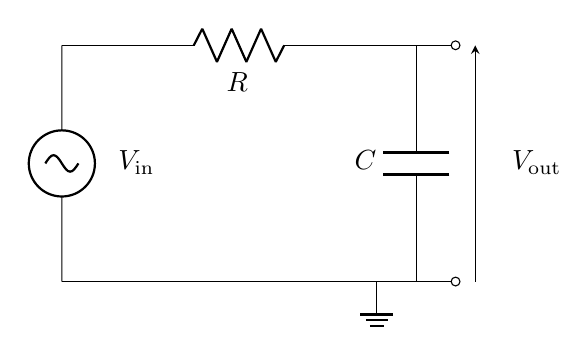
\begin{tikzpicture}[transform shape]
	% Paths, nodes and wires:
	\draw (1, 1) to[sinusoidal voltage source] (1, 4);
	\draw (1, 4) to[american resistor] (5.5, 4);
	\draw (5.5, 4) to[capacitor] (5.5, 1);
	\draw (5.5, 1) |- (1, 1);
	\node[ground] at (5, 1){};
	\node[shape=rectangle, minimum width=0.715cm, minimum height=0.715cm] at (1.875, 2.5){} node[anchor=north west, align=left, text width=0.327cm, inner sep=6pt] at (1.5, 2.875){$V_{\mathrm{in}}$};
	\node[shape=rectangle, minimum width=0.715cm, minimum height=0.715cm] at (3.25, 3.5){} node[anchor=north west, align=left, text width=0.327cm, inner sep=6pt] at (2.875, 3.875){$R$};
	\node[shape=rectangle, minimum width=0.715cm, minimum height=0.715cm] at (4.875, 2.5){} node[anchor=north west, align=left, text width=0.327cm, inner sep=6pt] at (4.5, 2.875){$C$};
	\draw (5.5, 4) -- (6, 4);
	\node[ocirc] at (6, 4){};
	\node[shape=rectangle, minimum width=0.715cm, minimum height=0.715cm] at (6.875, 2.5){} node[anchor=north west, align=left, text width=0.327cm, inner sep=6pt] at (6.5, 2.875){$V_{\mathrm{out}}$};
	\draw (5.5, 1) -- (6, 1);
	\node[ocirc] at (6, 1){};
	\draw[-stealth] (6.25, 1) -| (6.25, 4);
\end{tikzpicture}
    \caption{LPF回路}
    \label{fig.LPF回路}
\end{figure}
図\ref{fig.LPF回路}の\(V_{\mathrm{out}}\)について解析していく。

まずこの回路は抵抗器とキャパシタが直列に接続されていて、簡単に言えばその間の電圧が\(V_{\mathrm{out}}\)である。

直列接続では、インピーダンスも単に足し合わせればよいので、抵抗器とキャパシタを合わせたインピーダンスは\(Z_{R}+Z_{C}\)である。
\begin{align}
    Z_R + Z_C &= R + \dfrac{1}{j\omega C} \\
    &= R - j\dfrac{1}{\omega C}
\end{align}
今回の\(V_{\mathrm{out}}\)はキャパシタ両端間の電圧であるから\(\dot{V}_{C}\)を求めれば良い。 抵抗比と同様にしてインピーダンス比から電圧は求められる。\(\dot{V}_{C} = \tfrac{Z_{C}}{Z_{R}+Z_{C}}\dot{V}_{\mathrm{in}}\)。
\begin{align}
    \dot{V}_{C} &= \dfrac{Z_{C}}{Z_{R}+Z_{C}}\dot{V}_{\mathrm{in}} \\
    &= \dfrac{-j\dfrac{1}{\omega C}}{R-j\dfrac{1}{\omega C}}\dot{V}_{\mathrm{in}} \\
    &= \dfrac{1}{1 + j\omega RC}\dot{V}_{\mathrm{in}}
\end{align}
つまるところ
\begin{align}
    \dot{V}_{\mathrm{out}} &= \dfrac{1}{1 + j\omega RC}\dot{V}_{\mathrm{in}} \label{eq.LPFの特性}
\end{align}
である。これを踏まえて実際の出力波形はどうなるだろうか。\ref{eq.LPFの特性}に、\(\exp(j\omega t)\)を作用させて、虚部をとれば良い。
\begin{align}
    \Im\ab(\dot{V}_{\mathrm{out}}\exp(j\omega t)) &= \Im\ab(\dfrac{1}{1 + j\omega RC}\dot{V}_{\mathrm{in}}\exp(j\omega t)) \\
    &= \Im\ab(\dfrac{1}{1 + j\omega RC}V_{0}\exp(j \alpha)\exp(j\omega t)) \\
    &= \Im\ab(\dfrac{1}{1 + j\omega RC}V_{0}\exp(j(\omega t + \alpha))) \label{eq.インピを変換する前} \\
    &= \Im \ab(\sqrt{\dfrac{1+\ab(\omega RC)^2}{\ab(1+\ab(\omega RC)^2)^2}}V_0 \exp \ab(j \ab(\omega t + \alpha - \arctan (\omega RC)))) \label{eq.インピを変換した後}\\
    &= \sqrt{\dfrac{1}{1+\ab(\omega RC)^2}}V_0 \sin \ab(\omega t + \alpha - \arctan (\omega RC))
\end{align}
一応式変形の説明をすると\ref{eq.インピを変換する前}式から\ref{eq.インピを変換した後}式で、\(\tfrac{1}{1+j\omega RC}\)を指数表示に変換している。\(\tfrac{1}{1+j\omega RC} = \sqrt{\tfrac{1+\ab(\omega RC)^2}{\ab(1+\ab(\omega RC)^2)^2}}\exp\ab(-j \arctan (\omega RC))\)。

つまり出力振幅は入力電圧の振幅に対して\(\sqrt{\tfrac{1}{1+\ab(\omega RC)^2}}\)倍になっている。これを\(\omega\)の関数とみてグラフをかいたものが図\ref{fig.LPFのボード線図}である。角振動数が大きくなるほど、振幅が小さくなるような振る舞いが見られる。つまり、低い周波数ほどよく通す回路であり、そのためにローパスフィルターの名前をもつ。
\begin{figure}[htbp]
    \centering
    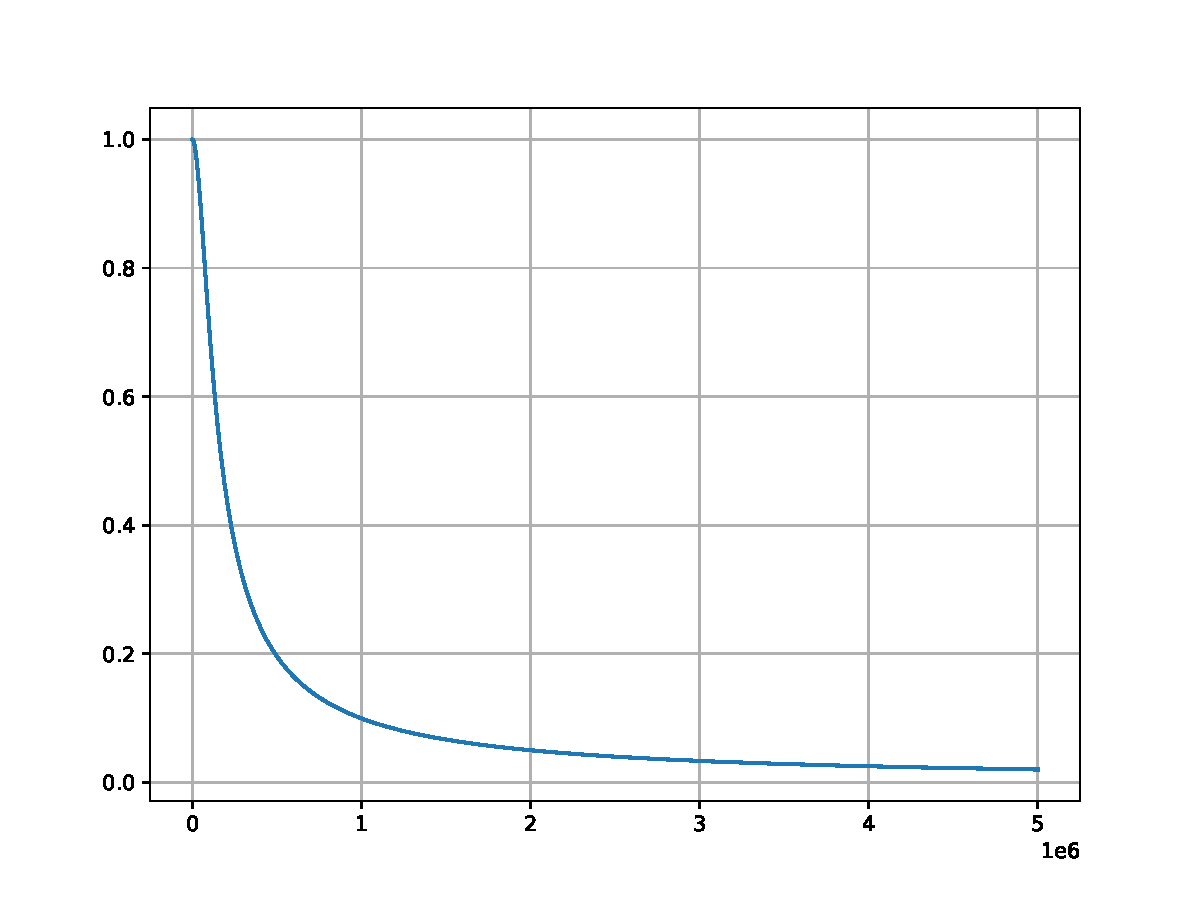
\includegraphics[width = 0.8\linewidth]{../lpf_graph.pdf}
    \caption{\(\sqrt{\tfrac{1}{1+\ab(\omega RC)^2}}\) vs \(\omega\)}
    \label{fig.LPFのボード線図}
\end{figure}

また出力電圧の位相をみると、入力に対して\(\arctan(\omega RC)\)だけ位相が遅れていることを示している。つまり、適当に抵抗器やキャパシタの抵抗値やキャパシタンスを変更すれば任意の位相差の信号を得られる。
\subsubsection{ハイパスフィルター(HPF)}
次にハイパスフィルターを同様に考えていく。ハイパスフィルターの例は次のような回路である。
\begin{figure}[htbp]
    \centering
    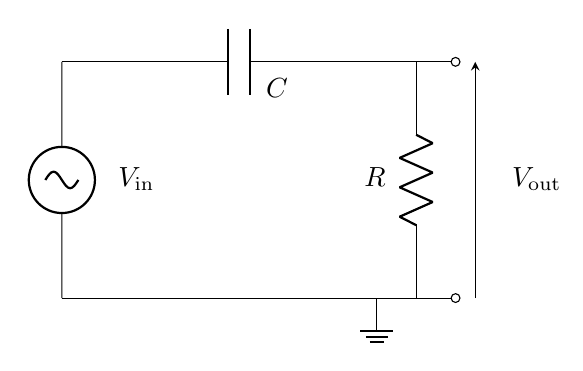
\begin{tikzpicture}[transform shape]
	% Paths, nodes and wires:
	\draw (1, 1) to[sinusoidal voltage source] (1, 4);
	\draw (5.5, 1) |- (1, 1);
	\node[ground] at (5, 1){};
	\node[shape=rectangle, minimum width=0.715cm, minimum height=0.715cm] at (1.875, 2.5){} node[anchor=north west, align=left, text width=0.327cm, inner sep=6pt] at (1.5, 2.875){$V_{\mathrm{in}}$};
	\node[shape=rectangle, minimum width=0.715cm, minimum height=0.715cm] at (5, 2.5){} node[anchor=north west, align=left, text width=0.327cm, inner sep=6pt] at (4.625, 2.875){$R$};
	\node[shape=rectangle, minimum width=0.715cm, minimum height=0.715cm] at (3.75, 3.625){} node[anchor=north west, align=left, text width=0.327cm, inner sep=6pt] at (3.375, 4){$C$};
	\draw (5.5, 4) -- (6, 4);
	\node[ocirc] at (6, 4){};
	\node[shape=rectangle, minimum width=0.715cm, minimum height=0.715cm] at (6.875, 2.5){} node[anchor=north west, align=left, text width=0.327cm, inner sep=6pt] at (6.5, 2.875){$V_{\mathrm{out}}$};
	\draw (5.5, 1) -- (6, 1);
	\node[ocirc] at (6, 1){};
	\draw[-stealth] (6.25, 1) -| (6.25, 4);
	\draw (1, 4) to[capacitor] (5.5, 4);
	\draw (5.5, 4) to[american resistor] (5.5, 1);
\end{tikzpicture}
    \caption{HPF回路}
    \label{fig.HPF回路}
\end{figure}
これはさっきのLPF回路の抵抗器とキャパシタを入れ替えたものになっている。

なので今度は抵抗器間電圧\(\dot{V}_{R}\)を求めれば良い、手順も全く同様である。

\begin{align}
    \dot{V}_R &= \dfrac{Z_R}{Z_R + Z_C}\dot{V}_{\mathrm{in}} \\
    &= \dfrac{j\omega RC}{1+j\omega RC}\dot{V}_{\mathrm{in}} \label{eq.HPFの特性}
\end{align}
また\ref{eq.HPFの特性}に\(\exp(j\omega t)\)を作用させて虚部をとる操作をすると
\begin{align}
    \Im \ab(\dot{V}_R\exp(j\omega t)) &= \Im \ab(\dfrac{j\omega RC}{1+j\omega RC}\dot{V}_{\mathrm{in}}\exp(j\omega t))
\end{align}
\subsubsection{共振回路}
\end{document}